When working with Level Sets you almost always work with small objects
in a much bigger world. This is due to the fact that our level set is
defined in global space, and we have to manipulate it in the complete
workspace to make sure the SDF is always welldefined, meaning the
length of the gradient is equal to one. This is a time consuming
process as described in section \vref{sec:reinitialize}. A solution to
make the processes faster is to only work on the areas of the SDF just
beside the contour of the level set we are working on. This method is
called the Narrow Band method and is described
in \cit{adalsteinsson1995fast}. A Narrow band of the Aarhus University logo can be seen in figure \vref{fig:nb-au-logo}.


\begin{figure}[h]
  \centering
  \subfloat[The interface]{
    
\includegraphics[width=0.3\textwidth]{imgs/nb-au}}
  \subfloat[The Narrow band]{
    
\includegraphics[width=0.3\textwidth]{imgs/nb-au-band}}

  \caption{Visualizing the Narrow band of the AU logo.}
  \label{fig:nb-au-logo}
\end{figure}

\subsection*{Idea of the Narrow Band Method}
The basic idea of the method is to narrow down the amount of pixels we
are working on, to include as few as possible without loosing
precision. This is done by keeping a band of $\gamma$ pixels around
the edges in SDF so we only update the SDF where
$\gamma \leq \phi(x,y) \leq \gamma$. When we solve the level set
equation within the narrow band, we use the values of the neighboring
pixels and as we can't trust the pixels outside our narrow band, we
have to do this in another way. This is where the outer band, also
called an safety band, comes in to play. All the neighbors on both
sides of our narrow band is added to this set. The outer band only job
is to supply the inner band with information when calculating on the
border of the band. Because we know how big $\gamma$ is, it is safe to
assume that the distance from the outer band to $\phi=0$ is more or
less $\gamma$. Setting the value of all pixels in the outer band to
$\gamma$ is therefore safe if we promise to reinitialize the band
afterwards to make the length of the gradients to become 1 again. This
will make the whole narrow band including the outer band satisfy the
requirements of the SDF and we only have to do inside the band
itself. Hence the program flow is changed a little. We first advect
the interface by solving the level set equation on the SDF. We then
recalibrate the narrow band to fit the newly generated SDF and
then at the end reinitialize it.


\begin{figure}[!ht]
  \centering
  \begin{tabular}{ | c | }
   \hline			
   Solve level set equation \\
   \hline
   Update narrow band \\
   \hline   
   Reinitialize \\
   \hline  
  \end{tabular}
  \caption{Program flow with Narrow band}
  \label{fig:narrowband_flow}
\end{figure}


To decide the size of $\gamma$, and thereby the width of the narrow
band, we have to look at the maximum distance the interface can move
in a time step. In our implementation this boundary is at one pixel
per time step, therefor a narrow band of size 3 around the interface
is sufficient. As seen in figure \vref{fig:nb-au-logo} the band
reaches just outside the interface border as displayed in red. The
green outline around the red band is the outer safe band.

\begin{figure}[h]
  \centering
  \subfloat[The output]{
    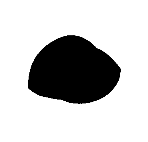
\includegraphics[width=0.3\textwidth]{imgs/nb1}}
  \subfloat[Without narrow band]{
    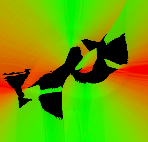
\includegraphics[width=0.3\textwidth]{imgs/nb2}}
  \subfloat[With narrow band]{
    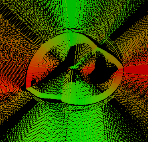
\includegraphics[width=0.3\textwidth]{imgs/nb3}}
  \caption{Same step while only reinitializing once per time step. Black in (b) and (c) represents an erroneous length of gradient.}
  \label{fig:narrowBand}
\end{figure}




\subsection{Implementation}


\subsection{Building the initial narrow band}
\begin{lstlisting}
    for (unsigned int x=0; x<width; x++)
        for (unsigned int y=0; y<height; y++) {
            float phiVal = fabs((*phi)(x, y));
            if (phiVal <= narrowBandWidth) {
                //Part of the inner band
                narrowBand[narrowBandSize++] = (Vector<3,int> (x,y));
                nbType(x,y) = 1;
            } else if (phiVal <= narrowBandWidth + 1.0f) {
                //Part of the outer(safety) band
                narrowBand[narrowBandSize++] = (Vector<3,int> (x,y));
                nbType(x,y) = 2;
            } else {
                nbType(x,y) = 0;
            }
        }
\end{lstlisting}

bbbbbbbbbb \cit{peng1999pde}

\subsection{Rebuilding the narrow band}
Rebuild Narrow Band

                %% if ((*phi)(x,y) >= 0)
                %%     (*phi)(x,y) = narrowBandWidth;
                %% else 
                %%     (*phi)(x,y) = -narrowBandWidth;



\missingfigure{Billede der viser et narrowband tæt på, med 3 i bredde og et safetybånd på 1 px.}

\subsection{Conclution}
\todoVester{Skriv NB Conclution}
